%------------------------------------------------------------------------------
%	CAPITOLO 40
%------------------------------------------------------------------------------

\chapter{Lisco}
Bumb... bumb... bumbum... l'è morto P\:.\:.\:. l'è morto P\:.\:.\:. bum... bum... bumbumb... ecc. col passo secco assordante di due zoccoli ferrati, si sentiva per la via. Era \index[Personaggi]{Lisco}Lisco, che passava a passo veloce per dare al paese un nuovo annunzio funebre.\\
E ciò appena era morto qualc'uno. Come facesse questo disgraziato a conoscere subite tutte le novità e specialmente quelle di morte, nessuno lo sapeva. Forse lo guidava un istinto di godimento per lo spettacolo del funerale nel quale era sempre in testa, specie se vi era la banda.\\
Nella sua idiozia maliziosa si sentiva ammirato e qualche cosa in queste funzioni... di male augurio. Gli annunzi funebri li proclamava coi panni da fatica, zoccoli, saccona, calzoni rimboccati, cappello rovesciato e fissato in testa sul tondello copri testa. Ai funerali precedeva tutti... al rombo della sera musica... e canto... sbirciando di traverso gli spettatori fermi sui marciapiedi. Lo seguiva uno stuolo di bambini.\\
Questo disgraziato, idiota, seguendo un funerale credeva d'andare alla festa... sfoggiando il vestito nuovo, con sul panciotto una catenella da sembrare il barbazzale\footnote{Catenella che unisce i due occhi del morso passando dietro la barbozza del cavallo} di un cavallo focoso.\\
Il suo linguaggio era tutto speciale: "siglio" per \emph{si}, "miglio" per \emph{me}, "iglei" per \emph{lei}, ecc. Non sapeva né il dialetto né l'italiano,,, che credeva d'inventare. Le comitive allegre lo fermavano e per l'esca di qualche soldo lo facevano dire il dizionario dei suoi sproloqui e ridevano.\\
Oltre che l'uomo del male augurio per gli annunzi funebri si era anche arrogato la specialità degli auguri di capo d'anno ed il suo da fare per questa impresa durava vari giorni.\\
Chi voleva ridere rispondeva al buon anno di \index[Personaggi]{Lisco}Lisco "grazie, altrettanto" ma \index[Personaggi]{Lisco}Lisco... subito: "datemi due soldi" e così passava tutti incassando qualche scudo.\\
Quando si presentò alla rivista militare fu pronto a spogliarsi, ma la commissione lo tenne in disparte per osservarlo meglio e chiesero informazioni al Sindaco presente. Il responso della Commissione di leva fu la classifica di 'idiota'.\\
A chi chiedeva a Lisco, che cosa voleva dire ‘idiota', con serietà rispondeva "vuglio dire miglio sono baibo" (io sono balbuziente).\\
Un giorno, col cappello rovesciato, gli zoccoli nei piedi e nella saccona infilato l'ombrello di tela cerata verde... battendo la sua solita musica, a \index[Luoghi]{Bologna}Bologna andò ad infilare via \index[Luoghi]{Rizzoli (via)}Rizzoli, seguito da uno stuolo di ragazzi che lo motteggiavano. La passeggiata finì, come doveva finire, fu preso dalle guardie e portato a vedere il cielo a scacchi\footnote{Portato in prigione}... per essere rimpatriato. Il bello però venne quando gli sequestrarono 12 scudi, frutto delle guardie. Montò su tutte le furie... ma le guardie sopraffecero e lo immobilizzarono... e lui ad urlare: "Lêdar dasim i mi bulèn!"\footnote{"Ladri datemi i miei soldi!"}\\
La sua deficienza mentale, lo salvò da altre pene... ed a \index[Luoghi]{Bologna}Bologna non andò più.\\

 \begin{figure}[htb]
    \centering
    %\vspace{-0.7cm}
    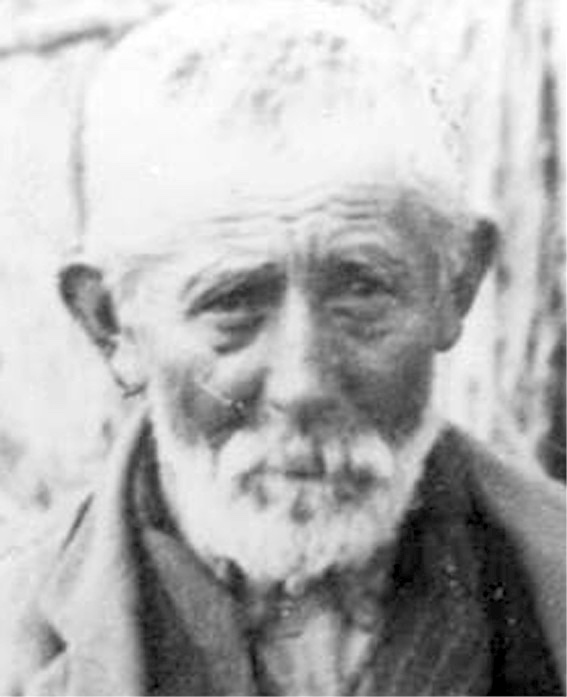
\includegraphics[height=8cm]{Lisco}
    \caption*{Lisco, ritratto da vecchio, personaggio famoso ad Alfonsine\label{fig:Lisco}}
    %\vspace{-0.3cm}
\end{figure}



